% !TEX program = xelatex
\documentclass[a4paper,10pt]{article}

\makeatletter
\let\@expl@@@mark@update@singlecol@structures@@\relax
\makeatother

\usepackage[a4paper, left=1.0cm, right=1.0cm, top=0.90cm, bottom=1.05cm, footskip=0.48cm]{geometry}
\usepackage{fontspec}
\usepackage{amsmath, amssymb}
\usepackage{array, colortbl}
\usepackage[table]{xcolor}
\usepackage{tcolorbox}
\tcbuselibrary{skins, breakable}
\usepackage{fancyhdr}
\usepackage{enumitem}
\usepackage{tikz}
\usetikzlibrary{calc, angles, quotes, arrows.meta}

\makeatletter
\newcommand{\NGSFindFonts}{%
  \IfFileExists{../../../fonts/KhmerOSsiemreap.ttf}{%
    \def\NGSUserPath{../../../fonts/}\def\NGSSysPath{../../../fonts/}%
  }{%
    \IfFileExists{../../../../fonts/KhmerOSsiemreap.ttf}{%
      \def\NGSUserPath{../../../../fonts/}\def\NGSSysPath{../../../../fonts/}%
    }{%
      \IfFileExists{fonts/KhmerOSsiemreap.ttf}{%
        \def\NGSUserPath{fonts/}\def\NGSSysPath{fonts/}%
      }{%
        \def\NGSUserPath{C:/Users/user/AppData/Local/Microsoft/Windows/Fonts/}%
        \def\NGSSysPath{C:/Windows/Fonts/}%
      }%
    }%
  }%
}
\NGSFindFonts
\makeatother

\XeTeXlinebreaklocale "km"
\XeTeXlinebreakskip = 0pt plus 1pt minus 0.1pt

\setmainfont[
  Path = {\NGSUserPath},
  Extension = .ttf,
  UprightFont = KhmerOSsiemreap,
  BoldFont = KhmerOSsiemreap,
  BoldFeatures = {FakeBold=1.8},
  ItalicFont = KhmerOSsiemreap,
  ItalicFeatures = {FakeSlant=0.25}
]{KhmerOSsiemreap}

\newfontfamily\muol[Path={\NGSUserPath}]{KhmerOSmuollight.ttf}
\newfontfamily\enfont[Path={\NGSSysPath}, Scale=1.0]{times.ttf}
\newfontfamily\enbold[Path={\NGSSysPath}, Scale=1.0]{timesbd.ttf}
\newfontfamily\calibrifont[Path={\NGSSysPath}, Scale=0.95]{calibri.ttf}

\DeclareTextFontCommand{\en}{\enfont}
\newcommand{\enbf}[1]{{\enbold #1}}

\definecolor{headgray}{HTML}{E2E2E2}
\definecolor{panelgray}{HTML}{F5F5F5}

\pagestyle{fancy}
\fancyhf{}
\renewcommand{\headrulewidth}{0pt}
\renewcommand{\footrulewidth}{0.4pt}
\fancyfoot[L]{\rule{0pt}{11pt}\fontsize{8.5pt}{11pt}\selectfont អនុវិទ្យាល័យព្រះក្រសាំង $\;\vert\;$ គណិតវិទ្យា ថ្នាក់ទី៨ $\;\vert\;$ មេរៀនទី១៥ (១៥.២.១) មុំផ្ចិត និងរង្វាស់ធ្នូ}
\fancyfoot[R]{\rule{0pt}{11pt}\fontsize{8.5pt}{11pt}\selectfont ទំព័រ \en{\thepage\,/\,2}}

\setlength{\parindent}{0pt}
\setlength{\tabcolsep}{4pt}

\newcommand{\tri}[1]{\triangle #1}
\newcommand{\unit}[1]{\,\text{\en{#1}}}
\newcommand{\blank}[1]{\leavevmode\hbox to #1{\dotfill}}
\newcommand{\chkbox}{\tikz[baseline=0.2ex]\draw[black, line width=0.7pt] (0,0) rectangle (1.55ex,1.55ex);}
\newcommand{\cnum}[1]{\tikz[baseline=-0.58ex]\node[circle, fill=black, text=white, inner sep=0.85pt, minimum size=1.95ex, font=\enbold\scriptsize]{#1};}

\newcommand{\arc}[1]{\mbox{%
  \tikz[baseline=(arcX.base)]{%
    \node[inner sep=0pt, outer sep=0pt] (arcX) {$#1$};%
    \draw[black, line width=0.55pt] ($(arcX.north west)+(0.02,0.035)$) to[bend left=30] ($(arcX.north east)+(-0.02,0.035)$);%
  }%
}}

\newcommand{\rightbox}[4][0.20cm]{%
  \coordinate (rbA) at ($(#3)!#1!(#2)$);
  \coordinate (rbB) at ($(#3)!#1!(#4)$);
  \coordinate (rbC) at ($(rbA)+(#3)!#1!(#4)-(#3)$);
  \draw[black, line width=0.65pt] (rbA) -- (rbC) -- (rbB);
}

\newcommand{\secbar}[2]{%
  \vspace{2.5pt}%
  \begin{tcolorbox}[
    enhanced, sharp corners, colback=headgray, colframe=black,
    boxrule=0.85pt, left=6pt, right=6pt, top=2.5pt, bottom=2.5pt, after skip=3.5pt
  ]
    {\muol\fontsize{9.5pt}{14pt}\selectfont #1}\hfill{\fontsize{9pt}{13pt}\selectfont\textbf{#2}}
  \end{tcolorbox}%
}

\begin{document}
\fontsize{9.6pt}{14.2pt}\selectfont

% ==================== ក្បាលសន្លឹកកិច្ចការ ====================
\begin{tcolorbox}[
  enhanced, sharp corners, colback=white, colframe=black,
  boxrule=1.1pt, left=6pt, right=6pt, top=3.5pt, bottom=3.5pt, after skip=3pt
]
  \begin{minipage}[c]{11.2cm}
    {\muol\fontsize{10.5pt}{15.5pt}\selectfont សន្លឹកកិច្ចការសិស្ស — មេរៀនទី១៥ ៖ រង្វង់}\\[1.5pt]
    \textbf{ចំណុចទី ២ ៖ មុំផ្ចិត រង្វាស់ធ្នូគិតជាដឺក្រេ និងប្រវែងធ្នូ} (សៀវភៅគោល ទំ.១៩៩--២០០)
  \end{minipage}\hfill
  \begin{minipage}[c]{6.7cm}
    ឈ្មោះសិស្ស៖ \blank{4.4cm}\\[2pt]
    ថ្នាក់ទី៨៖ \blank{1.3cm} \hspace{0.2cm} ដៃគូទី៖ \blank{2.0cm}
  \end{minipage}
\end{tcolorbox}

% ==================== ផ្នែកទី ១ ៖ E1 - ENGAGE ====================
\secbar{ផ្នែកទី ១ ៖ បេសកកម្មរហាត់ទឹកស្ទឹងសែន (\enbf{E1}) — រង្វង់រួមផ្ចិតពីរជាន់}{\en{3} នាទី (ទស្សន៍ទាយមុនរៀន)}

\begin{tcolorbox}[
  enhanced, sharp corners, colback=panelgray, colframe=black,
  boxrule=0.8pt, left=6pt, right=6pt, top=3pt, bottom=3pt, after skip=3pt
]
  \begin{minipage}[c]{12.3cm}
    ជាងធ្វើរហាត់ទឹកនៅដងស្ទឹងសែនពត់ខ្នងឫស្សីជារង្វង់រួមផ្ចិតពីរជាន់៖ ខ្នងក្នុងមានកាំ $r_1 = 1\unit{m}$ និងខ្នងក្រៅមានកាំ $r_2 = 2\unit{m}$។ ចន្លោះកាំឫស្សីពីរជាប់គ្នាបង្កើតបានមុំផ្ចិត $\angle xOy = 60^\circ$។ ចូរទស្សន៍ទាយ៖\\[2pt]
    ១. តើធ្នូក្នុង $\arc{A_1B_1}$ និងធ្នូក្រៅ $\arc{A_2B_2}$ មាន \textbf{រង្វាស់ដឺក្រេ} ស្មើគ្នាឬទេ? \hspace{0.12cm} \mbox{\chkbox\ ស្មើគ្នា} \hspace{0.18cm} \mbox{\chkbox\ មិនស្មើគ្នា}\\[2pt]
    ២. តើឫស្សីពត់តាម $\arc{A_1B_1}$ និង $\arc{A_2B_2}$ មាន \textbf{ប្រវែងម៉ែត្រ} ស្មើគ្នាឬទេ? \hspace{0.12cm} \mbox{\chkbox\ ស្មើគ្នា} \hspace{0.18cm} \mbox{\chkbox\ មិនស្មើគ្នា}
  \end{minipage}\hfill
  \begin{minipage}[c]{5.8cm}
    \centering
    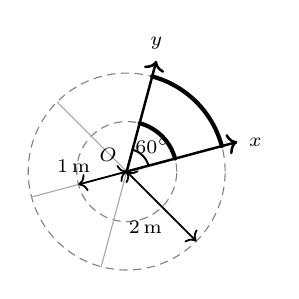
\begin{tikzpicture}[scale=0.41, every node/.style={font=\scriptsize, text=black}]
      \coordinate (O) at (0,0);
      \draw[black!50, densely dashed] (O) circle (1.55);
      \draw[black!50, densely dashed] (O) circle (3.05);
      \foreach \ang in {135,195,255,315} {\draw[black!35] (O)--(\ang:3.05);}
      \draw[black, line width=0.9pt, ->] (O)--(15:3.55) node[right=0.5pt] {$x$};
      \draw[black, line width=0.9pt, ->] (O)--(75:3.55) node[above=0.5pt] {$y$};
      \draw[black, line width=1.5pt] (15:1.55) arc (15:75:1.55);
      \draw[black, line width=1.5pt] (15:3.05) arc (15:75:3.05);
      \draw[black, line width=0.7pt] (15:0.70) arc (15:75:0.70);
      \node at (45:1.12) {$60^\circ$};
      \draw[black, line width=0.65pt, <->] (O)--(195:1.55);
      \node[above left=-1pt] at (195:0.95) {$1\unit{m}$};
      \draw[black, line width=0.65pt, <->] (O)--(-45:3.05);
      \node[below left=-1pt] at (-45:1.85) {$2\unit{m}$};
      \fill[black] (O) circle (2pt) (15:1.55) circle (1.8pt) (75:1.55) circle (1.8pt) (15:3.05) circle (1.8pt) (75:3.05) circle (1.8pt);
      \node[above left=0pt] at (O) {$O$};
    \end{tikzpicture}
  \end{minipage}
\end{tcolorbox}

% ==================== ផ្នែកទី ២ ៖ E2 - EXPLORE ====================
\secbar{ផ្នែកទី ២ ៖ ការរុករកមុំផ្ចិត កាដ្រង់ និងតារាងសមាមាត្រប្រវែងធ្នូ (\enbf{E2 — Explore})}{\en{11} នាទី (ពិភាក្សាដៃគូ)}

\textbf{(ក) មុំផ្ចិតលយ មុំផ្ចិតឆក និងកាដ្រង់ (ឧទាហរណ៍ទី១--៣ ទំ.១៩៩)៖} ពិនិត្យរូបទាំងពីរ រួចបំពេញចន្លោះ៖\\[2pt]
\begin{minipage}[c]{7.5cm}
  \centering
  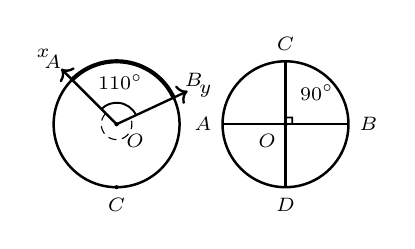
\begin{tikzpicture}[scale=0.39, every node/.style={font=\scriptsize, text=black}]
    \begin{scope}[shift={(0,0)}]
      \coordinate (O) at (2.3,2.3);
      \draw[black, line width=0.9pt] (O) circle (2.05);
      \draw[black, line width=1.5pt] ($(O)+(25:2.05)$) arc (25:135:2.05);
      \draw[black, line width=0.85pt, ->] (O)--($(O)+(25:2.55)$) node[right=0.5pt] {$y$};
      \draw[black, line width=0.85pt, ->] (O)--($(O)+(135:2.55)$) node[above left=0.5pt] {$x$};
      \draw[black, line width=0.7pt] ($(O)+(25:0.70)$) arc (25:135:0.70);
      \draw[black, densely dashed] ($(O)+(135:0.50)$) arc (135:385:0.50);
      \fill[black] (O) circle (2pt) ($(O)+(135:2.05)$) circle (1.9pt) ($(O)+(25:2.05)$) circle (1.9pt) ($(O)+(-90:2.05)$) circle (1.9pt);
      \node[below right=0pt] at (O) {$O$};
      \node[above left=0.5pt] at ($(O)+(135:2.05)$) {$A$};
      \node[above right=0.5pt] at ($(O)+(25:2.05)$) {$B$};
      \node[below=0.5pt] at ($(O)+(-90:2.05)$) {$C$};
      \node[above=1pt] at ($(O)+(80:0.72)$) {$110^\circ$};
    \end{scope}
    \begin{scope}[shift={(5.5,0)}]
      \coordinate (O2) at (2.3,2.3);
      \draw[black, line width=0.9pt] (O2) circle (2.05);
      \draw[black, line width=0.85pt] ($(O2)+(-2.05,0)$)--($(O2)+(2.05,0)$) ($(O2)+(0,-2.05)$)--($(O2)+(0,2.05)$);
      \rightbox[0.22cm]{$(O2)+(2.05,0)$}{O2}{$(O2)+(0,2.05)$}
      \fill[black] (O2) circle (2pt);
      \node[left=0.5pt] at ($(O2)+(-2.05,0)$) {$A$}; \node[right=0.5pt] at ($(O2)+(2.05,0)$) {$B$};
      \node[above=0.5pt] at ($(O2)+(0,2.05)$) {$C$}; \node[below=0.5pt] at ($(O2)+(0,-2.05)$) {$D$};
      \node[below left=0pt] at (O2) {$O$};
      \node at ($(O2)+(45:1.45)$) {$90^\circ$};
    \end{scope}
  \end{tikzpicture}
\end{minipage}\hfill
\begin{minipage}[c]{11.0cm}
  \begin{enumerate}[label=\enbf{\arabic*.}, leftmargin=1.4em, itemsep=2.5pt, topsep=1pt]
    \item មុំដែលមានកំពូលត្រង់ផ្ចិត $O$ នៃរង្វង់ហៅថា \textbf{មុំ\blank{1.6cm}} ហើយ $A, B$ ជា \textbf{ចុងធ្នូ}។
    \item បើមុំលយ $\angle xOy = 110^\circ$ (ស្កាត់ធ្នូតូច $\arc{AB}$) នោះមុំឆក $\angle xOy$ (ស្កាត់ធ្នូធំ $\arc{ACB}$) មានរង្វាស់ $360^\circ - 110^\circ =$ \blank{1.4cm}$^\circ$។
    \item បើអង្កត់ផ្ចិត $AB \perp CD$ រង្វង់ត្រូវចែកជា $4$ \textbf{\blank{1.9cm}} ប៉ុនៗគ្នា ដែលធ្នូនីមួយៗមានរង្វាស់ \blank{1.2cm}$^\circ$ (ឯកន្លះរង្វង់មានរង្វាស់ \blank{1.2cm}$^\circ$)។
  \end{enumerate}
\end{minipage}

\vspace{3pt}
\textbf{(ខ) តារាងសមាមាត្ររកប្រវែងធ្នូនៃរង្វង់កាំ $r$ (បរិមាត្ររង្វង់ពេញ $P = 2\pi r$)៖}\\[2pt]
\renewcommand{\arraystretch}{1.24}
\begin{tabular}{|p{3.9cm}|p{2.5cm}|p{2.9cm}|p{8.5cm}|}
  \hline
  \cellcolor{headgray}\centering\textbf{ផ្នែកនៃរង្វង់} &
  \cellcolor{headgray}\centering\textbf{មុំផ្ចិត ($\alpha$)} &
  \cellcolor{headgray}\centering\textbf{រង្វាស់ធ្នូ (ដឺក្រេ)} &
  \cellcolor{headgray}\centering\arraybackslash\textbf{ប្រវែងធ្នូ $l$ ធៀបនឹងបរិមាត្ររង្វង់ $P = 2\pi r$} \\[2pt]
  \hline
  រង្វង់ពេញ ១ ជុំ & \centering $360^\circ$ & \centering $360^\circ$ & \arraybackslash $l = P = 2\pi r$ \\[2pt]
  \hline
  កន្លះរង្វង់ ($\frac{1}{2}$ រង្វង់) & \centering $180^\circ$ & \centering \blank{1.3cm}$^\circ$ & \arraybackslash $l = \dfrac{P \times 180^\circ}{360^\circ} = \dfrac{1}{2}P = \pi r$ \\[3pt]
  \hline
  ១ កាដ្រង់ ($\frac{1}{4}$ រង្វង់) & \centering $90^\circ$ & \centering \blank{1.3cm}$^\circ$ & \arraybackslash $l = \dfrac{P \times 90^\circ}{360^\circ} =$ \blank{1.2cm} $\times P$ \\[3pt]
  \hline
  ធ្នូស្កាត់ដោយមុំ $1^\circ$ & \centering $1^\circ$ & \centering $1^\circ$ & \arraybackslash $l_1 = \dfrac{P}{360^\circ} = \dfrac{2\pi r}{360^\circ}$ \\[3pt]
  \hline
  \textbf{ធ្នូស្កាត់ដោយមុំ $\alpha^\circ$} & \centering $\alpha^\circ$ & \centering \blank{1.3cm}$^\circ$ & \arraybackslash $l = \dfrac{P \times \alpha}{360^\circ} = \dfrac{2\pi r \times \blank{1.2cm}}{360^\circ}$ \\[4pt]
  \hline
\end{tabular}

% ==================== ផ្នែកទី ៣ ៖ E3 - EXPLAIN ====================
\secbar{ផ្នែកទី ៣ ៖ សំយោគទ្រឹស្ដីបទមុំផ្ចិត និងការញែកដឺក្រេធ្នូ ទល់នឹង ប្រវែងធ្នូ (\enbf{E3 — Explain})}{\en{6} នាទី}

\begin{tcolorbox}[
  enhanced, sharp corners, colback=white, colframe=black,
  boxrule=1.0pt, boxsep=2pt, top=3.5pt, bottom=3.5pt, left=6pt, right=6pt, after skip=3.5pt
]
  $\bullet$ \textbf{ជាទូទៅ (ទំ.១៩៩)៖} នៅក្នុងរង្វង់តែមួយ (ឬរង្វង់ពីរប៉ុនគ្នា)៖\\
  \hspace*{0.4cm} ១. ធ្នូពីរប៉ុនគ្នា ស្កាត់ដោយមុំផ្ចិតពីរ \textbf{\blank{2.2cm}} ហើយមុំផ្ចិតពីរប៉ុនគ្នា ស្កាត់ធ្នូពីរ \textbf{\blank{2.2cm}} ($\arc{AB} = \arc{DE} \Leftrightarrow \angle AOB = \angle DOE$)។\\
  \hspace*{0.4cm} ២. ធ្នូពីរមិនប៉ុនគ្នា ធ្នូដែលធំជាង ស្កាត់ដោយមុំផ្ចិត \textbf{\blank{2.2cm}} ($\arc{CD} > \arc{AB} \Leftrightarrow \angle COD > \angle AOB$)។\\[2.5pt]
  $\bullet$ \textbf{រូបមន្តសំខាន់ទាំងពីរ៖} \textbf{(ក) រង្វាស់ធ្នូគិតជាដឺក្រេ៖} $\text{រង្វាស់ }\arc{AB} = \angle AOB = \alpha^\circ$ \textit{(មិនអាស្រ័យលើកាំ $r$ ទេ!)} $\;\vert\;$
  \textbf{(ខ) ប្រវែងធ្នូ៖} $l = \dfrac{2\pi r \times \alpha}{360^\circ}$ \textit{(គិតជាខ្នាតប្រវែង $\unit{cm}, \unit{dm}, \unit{m}$ និងប្រែប្រួលតាមកាំ $r$!)}។
\end{tcolorbox}

\begin{tcolorbox}[
  enhanced, sharp corners, colback=panelgray, colframe=black,
  boxrule=0.85pt, left=6pt, right=6pt, top=3pt, bottom=3pt
]
  \textbf{ផ្ទៀងផ្ទាត់ការយល់ដឹងភ្លាមៗ (គូសធីក \chkbox\ ពិត ឬ មិនពិត)៖}\\[2pt]
  ១. ធ្នូ $1^\circ$ ជាធ្នូដែលស្កាត់ដោយមុំផ្ចិតមានរង្វាស់ស្មើនឹង $1^\circ$។ \hfill \chkbox\ ពិត \hspace{0.35cm} \chkbox\ មិនពិត\\[2pt]
  ២. រង្វង់ពីរមានកាំខុសគ្នា ($r_1 = 3\unit{cm},\; r_2 = 6\unit{cm}$) បើមានមុំផ្ចិត $45^\circ$ ស្មើគ្នា នោះប្រវែងធ្នូទាំងពីរស្មើសង់ទីម៉ែត្រគ្នា។ \hfill \chkbox\ ពិត \hspace{0.35cm} \chkbox\ មិនពិត
\end{tcolorbox}

\newpage

% ==================== ទំព័រទី ២ ៖ E4, E5 និងកិច្ចការផ្ទះ ====================
\secbar{ផ្នែកទី ៤ ៖ ការអនុវត្តលំហាត់គំរូគណនាប្រវែងធ្នូ (\enbf{E4 — Elaborate})}{\en{10} នាទី (ទំ.១៩៩--២០០)}

\begin{tcolorbox}[
  enhanced, sharp corners, colback=white, colframe=black,
  boxrule=0.95pt, boxsep=2pt, top=4pt, bottom=4pt, left=6pt, right=6pt, after skip=4.5pt
]
  \begin{minipage}[c]{12.4cm}
    \textbf{១. លំហាត់គំរូទី ១ (ទំ.១៩៩--២០០)៖} រង្វង់មួយមានកាំ $r = 10\unit{dm}$។ គណនាប្រវែងធ្នូគិតជាដេស៊ីម៉ែត្រ ($\unit{dm}$) ដែលស្កាត់ដោយមុំផ្ចិត $\alpha = 36^\circ$ (យក $\pi \approx 3.14$)៖
    \begin{itemize}[leftmargin=1.2em, itemsep=3pt, topsep=2pt]
      \item បរិមាត្ររង្វង់ពេញ ($360^\circ$)៖ $P = 2\pi r = 2 \times 3.14 \times$ \blank{1.2cm} $=$ \blank{1.8cm} $\unit{dm}$។
      \item ប្រវែងធ្នូស្កាត់ដោយមុំ $1^\circ$ គឺ៖ $\dfrac{P}{360^\circ} = \dfrac{\blank{1.6cm}}{360^\circ}\;(\unit{dm})$។
      \item ប្រវែងធ្នូស្កាត់ដោយមុំ $36^\circ$ គឺ៖ $l = \dfrac{\blank{1.35cm} \times 36^\circ}{360^\circ} = \dfrac{\blank{1.35cm}}{10} =$ \blank{1.55cm} $\unit{dm}$។
    \end{itemize}
  \end{minipage}\hfill
  \begin{minipage}[c]{5.5cm}
    \centering
    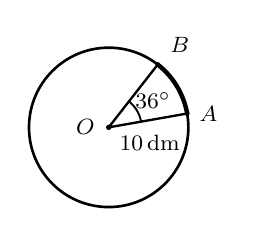
\begin{tikzpicture}[scale=0.44, every node/.style={font=\footnotesize, text=black}]
      \coordinate (O) at (0,0);
      \draw[black, line width=0.95pt] (O) circle (2.3);
      \draw[black, line width=1.6pt] (10:2.3) arc (10:52:2.3);
      \draw[black, line width=0.85pt] (O)--(10:2.3) (O)--(52:2.3);
      \draw[black, line width=0.7pt] (10:0.95) arc (10:52:0.95);
      \fill[black] (O) circle (2.2pt) (10:2.3) circle (2pt) (52:2.3) circle (2pt);
      \node[left=1.5pt] at (O) {$O$};
      \node[right=1pt] at (10:2.3) {$A$};
      \node[above right=1pt] at (52:2.3) {$B$};
      \node at (31:1.50) {$36^\circ$};
      \node[below=2pt] at (10:1.2) {$10\unit{dm}$};
    \end{tikzpicture}
  \end{minipage}
\end{tcolorbox}

\begin{tcolorbox}[
  enhanced, sharp corners, colback=white, colframe=black,
  boxrule=0.95pt, boxsep=2pt, top=4pt, bottom=4pt, left=6pt, right=6pt, after skip=4.5pt
]
  \begin{minipage}[c]{12.4cm}
    \textbf{២. លំហាត់គំរូទី ២ (ទំ.២០០)៖} រង្វង់មួយមានកាំ $r = 15\unit{cm}$ (យក $\pi = 3.14$)។ គណនាប្រវែងធ្នូ $\arc{AB}$ ដែលមានរង្វាស់ $80^\circ$ គិតជាសង់ទីម៉ែត្រ ($\unit{cm}$)៖
    \begin{itemize}[leftmargin=1.2em, itemsep=3pt, topsep=2pt]
      \item បរិមាត្ររង្វង់ ($360^\circ$)៖ $P = 2\pi r = 2 \times 3.14 \times$ \blank{1.2cm} $=$ \blank{1.8cm} $\unit{cm}$។
      \item រូបមន្តប្រវែងធ្នូ $80^\circ$៖ $l = \dfrac{P \times \alpha}{360^\circ} = \dfrac{\blank{1.6cm} \times 80^\circ}{360^\circ} = \dfrac{\blank{1.6cm} \times 2}{9}$។
      \item គណនាតម្លៃប្រហែលត្រឹមភាគរយ៖ $l \approx$ \blank{2.2cm} $\unit{cm}$។
    \end{itemize}
  \end{minipage}\hfill
  \begin{minipage}[c]{5.5cm}
    \centering
    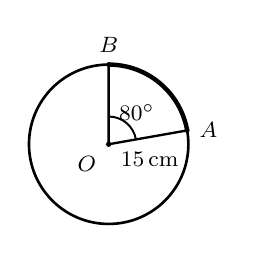
\begin{tikzpicture}[scale=0.44, every node/.style={font=\footnotesize, text=black}]
      \coordinate (O) at (0,0);
      \draw[black, line width=0.95pt] (O) circle (2.3);
      \draw[black, line width=1.6pt] (10:2.3) arc (10:90:2.3);
      \draw[black, line width=0.85pt] (O)--(10:2.3) (O)--(90:2.3);
      \draw[black, line width=0.7pt] (10:0.80) arc (10:90:0.80);
      \fill[black] (O) circle (2.2pt) (10:2.3) circle (2pt) (90:2.3) circle (2pt);
      \node[below left=1pt] at (O) {$O$};
      \node[right=1pt] at (10:2.3) {$A$};
      \node[above=1pt] at (90:2.3) {$B$};
      \node at (48:1.22) {$80^\circ$};
      \node[below=2pt] at (10:1.2) {$15\unit{cm}$};
    \end{tikzpicture}
  \end{minipage}
\end{tcolorbox}

% ==================== ផ្នែកទី ៥ ៖ E5 - EVALUATE ====================
\secbar{ផ្នែកទី ៥ ៖ ប្រតិបត្តិ លំហាត់ទី១ និងការបិទបេសកកម្ម (\enbf{E5 — Evaluate})}{\en{10} នាទី (ទំ.២០០ និង ២០៤)}

\begin{tcolorbox}[
  enhanced, sharp corners, colback=white, colframe=black,
  boxrule=0.95pt, boxsep=2pt, top=4pt, bottom=4pt, left=6pt, right=6pt, after skip=4.5pt
]
  \renewcommand{\arraystretch}{1.22}
  \begin{tabular}{|p{8.7cm}|p{8.7cm}|}
    \hline
    \cellcolor{headgray}\centering\textbf{១. ប្រតិបត្តិ (ទំ.២០០ — ប្រៀបធៀបមុំផ្ចិត)} &
    \cellcolor{headgray}\centering\arraybackslash\textbf{២. លំហាត់ទី ១ (ទំ.២០៤ — គណនារង្វាស់ធ្នូ)} \\[2pt]
    \hline
    \begin{minipage}[t]{8.5cm}
      \vspace{2pt}
      \begin{minipage}[c]{3.3cm}
        \centering
        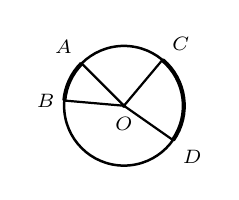
\begin{tikzpicture}[scale=0.38, every node/.style={font=\scriptsize, text=black}]
          \coordinate (O) at (0,0);
          \draw[black, line width=0.9pt] (O) circle (2.0);
          \draw[black, line width=1.5pt] (135:2.0) arc (135:175:2.0);
          \draw[black, line width=1.5pt] (-35:2.0) arc (-35:50:2.0);
          \draw[black, line width=0.8pt] (O)--(135:2.0) (O)--(175:2.0) (O)--(-35:2.0) (O)--(50:2.0);
          \fill[black] (O) circle (2pt);
          \node[below=0.5pt] at (O) {$O$};
          \node[above left=0pt] at (135:2.0) {$A$}; \node[left=0pt] at (175:2.0) {$B$};
          \node[above right=0pt] at (50:2.0) {$C$}; \node[below right=0pt] at (-35:2.0) {$D$};
        \end{tikzpicture}
      \end{minipage}\hfill
      \begin{minipage}[c]{5.0cm}
        ក្នុងរង្វង់ $C(O,r)$ ធ្នូតូចពីរមិនប៉ុនគ្នា៖ $\arc{AB} < \arc{CD}$។\\
        $\bullet$ ប្រៀបធៀបមុំផ្ចិត៖\\
        $\angle AOB$ \blank{0.9cm} $\angle COD$\\
        ព្រោះធ្នូតូចជាងស្កាត់ដោយមុំផ្ចិត \blank{1.9cm}។
      \end{minipage}
      \vspace{2pt}
    \end{minipage}
    &
    \arraybackslash
    \begin{minipage}[t]{8.5cm}
      \vspace{2pt}
      \begin{minipage}[c]{3.3cm}
        \centering
        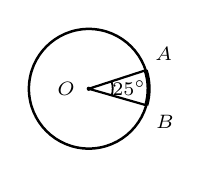
\begin{tikzpicture}[scale=0.38, every node/.style={font=\scriptsize, text=black}]
          \coordinate (O) at (0,0);
          \draw[black, line width=0.9pt] (O) circle (2.0);
          \draw[black, line width=1.5pt] (-16:2.0) arc (-16:18:2.0);
          \draw[black, line width=0.8pt] (O)--(-16:2.0) (O)--(18:2.0);
          \draw[black, line width=0.65pt] (-16:0.80) arc (-16:18:0.80);
          \fill[black] (O) circle (2pt);
          \node[left=1.5pt] at (O) {$O$};
          \node[above right=0pt] at (18:2.0) {$A$}; \node[below right=0pt] at (-16:2.0) {$B$};
          \node at (1:1.35) {$25^\circ$};
        \end{tikzpicture}
      \end{minipage}\hfill
      \begin{minipage}[c]{5.0cm}
        គេឱ្យមុំផ្ចិតលយ $\angle AOB = 25^\circ$។\\
        $\bullet$ រង្វាស់ធ្នូតូច $\arc{AB} =$ \blank{1.3cm}$^\circ$\\
        $\bullet$ រង្វាស់ធ្នូធំដែលនៅសល់គឺ៖\\
        $360^\circ - 25^\circ =$ \blank{1.4cm}$^\circ$។
      \end{minipage}
      \vspace{2pt}
    \end{minipage} \\[3pt]
    \hline
  \end{tabular}
\end{tcolorbox}

\begin{tcolorbox}[
  enhanced, sharp corners, colback=white, colframe=black,
  boxrule=0.95pt, boxsep=2pt, top=3.5pt, bottom=3.5pt, left=6pt, right=6pt, after skip=4.5pt
]
  \textbf{៣. បិទបេសកកម្ម E1 (រហាត់ទឹកស្ទឹងសែន $r_1=1\unit{m}, r_2=2\unit{m}, \alpha=60^\circ$)៖}\\
  $\bullet$ រង្វាស់ដឺក្រេ៖ $\arc{A_1B_1} =$ \blank{1.1cm}$^\circ$ និង $\arc{A_2B_2} =$ \blank{1.1cm}$^\circ$ (ស្មើគ្នា!)។ តែប្រវែងឫស្សី៖ $l_1 = \frac{2\times 3.14\times 1\times 60^\circ}{360^\circ} \approx$ \blank{1.4cm} $\unit{m}$ ឯ $l_2 \approx$ \blank{1.4cm} $\unit{m}$ ($= 2l_1$)!\\[3pt]
  \textbf{៤. Exit Check (៦០ វិនាទី)៖} រង្វង់រួមផ្ចិតពីរមានកាំ $r_1 = 5\unit{cm}$ និង $r_2 = 10\unit{cm}$ ស្កាត់ដោយមុំផ្ចិត $72^\circ$ រួមគ្នា។ តើអំណះអំណាងណាមួយត្រឹមត្រូវ?\\
  \chkbox\ \textbf{A.} ដឺក្រេធ្នូស្មើគ្នា ($72^\circ$) តែ $l_2 = 2l_1$ \hspace{0.35cm}
  \chkbox\ \textbf{B.} ប្រវែងធ្នូស្មើគ្នា ($l_1 = l_2$) \hspace{0.35cm}
  \chkbox\ \textbf{C.} ធ្នូក្រៅមានរង្វាស់ $144^\circ$ \hspace{0.35cm}
  \chkbox\ \textbf{D.} $l_1 = 2l_2$
\end{tcolorbox}

% ==================== កិច្ចការផ្ទះ (ជំហានទី ៥) ====================
\begin{tcolorbox}[
  enhanced, sharp corners, colback=panelgray, colframe=black,
  boxrule=1.0pt, boxsep=2pt, top=3.5pt, bottom=3.5pt, left=6pt, right=6pt
]
  {\muol\fontsize{9.0pt}{13pt}\selectfont កិច្ចការផ្ទះ (ពង្រឹងលំហាត់ទី១ ទំព័រ ២០៤ និងត្រៀមអានចំណុច ២.១ ទំព័រ ២០០--២០១)}\\[2pt]
  $\bullet$ \textbf{លំហាត់ ១៖} ក្នុងរង្វង់ $C(O, 18\unit{cm})$ គេមានមុំផ្ចិត $\angle AOB = 25^\circ$ និង $\angle COD = 120^\circ$។ ចូរគណនារង្វាស់ដឺក្រេនៃធ្នូធំ $\arc{ACB}$ និងគណនាប្រវែងធ្នូតូច $\arc{AB}$ ព្រមទាំងធ្នូតូច $\arc{CD}$ គិតជា $\unit{cm}$ (យក $\pi \approx 3.14$)។\\
  $\bullet$ \textbf{លំហាត់ ២ (ចំណោទច្រាស)៖} ធ្នូតូច $\arc{MN}$ មួយនៅលើរង្វង់កាំ $r = 15\unit{cm}$ មានប្រវែង $l = 15.7\unit{cm}$ ($\pi \approx 3.14$)។ ចូរគណនារង្វាស់មុំផ្ចិត $\angle MON$ គិតជាដឺក្រេ។
\end{tcolorbox}

\end{document}
